%!TEX root = ../thesis.tex
%*******************************************************************************
%****************************** Fifth Chapter **********************************
%*******************************************************************************
\chapter{Neuromorphic Modelling Framework}

\section[Optically Active Device]{Optically Active Device}

This chapter presents a model for resistance switching devices that demonstrates both analogue potentiation and conductance depression under the same voltage polarity, exploring the subthreshold regime with current transients, which has the potential to simplify neuromorphic circuits. The utilisation of an empirical SPICE model enables the simulation of these transients, with the process of validation being achieved through the use of experimental data. \\

\noindent This provides parameters for reader simulations and facilitates applications such as fault mobility estimation and neuromorphic circuit functions. The enhancements made to the previous model include the integration of diodes to emulate Schottky-like contact and the incorporation of relaxation dynamics upon the removal of step potentials or the grounding of the device.

\subsection[Modified Device Stack]{Modified Device Stack}

A distinct set of devices with disparate top electrical contacts were characterised, one with conductive indium tin oxide (ITO) in lieu of gold. The bottom contact and oxide layer remained unaltered and consistent with those observed in the gold-contacted devices presented in the preceding section. When subjected to stress, the ITO-contacted device exhibited a distinct response compared to the gold-titanium contacted device. Instead of a gradual and smooth increase in conductance, the response was more erratic and chaotic. \\

\begin{table}[ht]
    \caption{Comparison of the modified device stacks.}
    \centering
    \begin{tabular}{|cc|cc|}
    \hline
    \multicolumn{2}{|c|}{Original Stack}              & \multicolumn{2}{c|}{Modified Stack}              \\ \hline
    \multicolumn{1}{|c|}{Layer} & Film Thickness (nm) & \multicolumn{1}{c|}{Layer} & Film Thickness (nm) \\ \hline
    \multicolumn{1}{|c|}{Au}    & 110                 & \multicolumn{1}{c|}{ITO}   & 30                  \\ \hline
    \multicolumn{1}{|c|}{Ti}    & 3                   & \multicolumn{1}{c|}{Ti}    & 3                   \\ \hline
    \multicolumn{1}{|c|}{SiOx}  & 35                  & \multicolumn{1}{c|}{SiOx}  & 20                  \\ \hline
    \multicolumn{1}{|c|}{Mo}    & 280                 & \multicolumn{1}{c|}{Mo}    & 150                 \\ \hline
    \end{tabular}
    \label{table:5a}
\end{table}
    
\noindent The aluminium-contacted devices have yet to demonstrate the occurrence of current transients following the application of stress. In addition to failing to exhibit current transients, any increase in conductance induced by the constant current stress is also observed to be more volatile than that observed in the other devices, with the devices returning to a high resistance state within a couple of hours.\\


\noindent The aluminium-contacted devices have yet to demonstrate the occurrence of current transients following the application of stress. In addition to failing to exhibit current transients, any increase in conductance induced by the constant current stress is also observed to be more volatile than that observed in the other devices, with the devices returning to a high resistance state within a couple of hours.\\

\begin{figure}[htbp!] 
\centering    
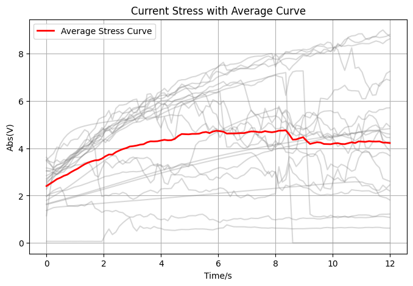
\includegraphics[width=0.6\textwidth]{Chapter5/Figs/a.png}
\caption[Stressing responses of ITO top contacted device.]{Stressing responses of ITO top contacted device. With the objective to ascertain the stress responses of the ITO top-contacted device, the voltage across the device was monitored while it was subjected to a constant current of $-0.5\mu A$. It was not possible to apply larger currents. The response was observed to be less smooth when compared to that of the gold-contacted device.}
\label{fig:5a}
\end{figure}

\noindent In contrast, the ITO contacted devices did exhibit transients, but interestingly, only partially. A typical transient observed in ITO devices is plotted in Figure \ref{fig:5a}. It exhibits the initial increase in conductance as is typical with current transients, but does not then start reducing in conductance. Instead, the device exhibits a chaotic spiking-like behaviour which, if observed for too long, will cause the device to switch to a low resistance state.\\

\noindent The observation of a partial current transient in ITO-contacted devices is a significant finding. As will be discussed in the following section, this evidence is indicative of the transient being the result of multiple simultaneous changes occurring in the device. Furthermore, it supports the hypothesis that the top metal-insulator interface plays a role in generating transients.\\

\noindent The hypothesis that alterations to specific interfaces of the device can influence the characteristics of the current transient is supported by findings in tantalum oxide-based devices \cite{tuller2011point}. In this study, a layer of $Al_2O_3$ was deposited between the tantalum oxide bulk and the titanium nitride electrodes, which reduced the prominence of the current transient in the absence of the buffer layer.\\

\noindent To illustrate, the gradual decline in conductance of the transients is exclusive to the gold-contacted device, indicating that it is either due to the characteristics of the metal-insulator interface or the disparate responses to stressing at this interface that determine whether the decaying behaviour is manifested. \\

\noindent In contrast, the initial increase in conduction is observed in both the ITO and gold-contacted devices. This suggests that the behaviour is less affected by the top metal-insulator interface and may be located in the bulk oxide layer or at the bottom metal-insulator interface. The disappearance of the slower decay in conductance with the change in top electrode may provide insight into the physical model describing the current change. 


\subsection[Conductance Variation Mechanisms]{Conductance Variation Mechanisms}

The initial step is to ascertain the location within the device stack where alterations are taking place that are responsible for the observed reduction in conductance. The absence of decay occurring concurrently with the alteration of the top electrode suggests that the causal factor responsible for the observed conductance decay is situated at the interface between the top electrode and the amorphous silicon dioxide. \\

\noindent Given the slow dynamics of the change in conductance, it is plausible that a drift of some mobile defect is responsible. It is well established that silicon dioxide films are susceptible to the influence of alkali mobile ions \cite{snow1965ion}, including sodium and lithium ions, which are all characterised by a positive charge \cite{yon1966sodium}. The drift of these mobile charges can significantly affect the potential drops at metal-oxide interfaces, as well as modulate barrier heights when allowed to accumulate.\\

\noindent If some positive mobile ion, regardless of the species, existed in the oxide of the device, it would be attracted to the top electrode, which is at a negative potential. This would cause an accumulation of positive space charge at the interface, which would in turn reduce the potential across the oxide. Nevertheless, it can be argued that alkali metals, such as sodium and potassium, are unlikely to be the cause of this positive space charge, given that they do not migrate at room temperature. \\

\noindent Instead, they require temperatures in excess of 100 degrees Celsius (212 degrees Fahrenheit) \cite{deal1974current}. The current transients presented in this thesis are all observed at room temperature, which suggests the need for an alternative candidate to explain the mobile space charge, in particular one that is mobile at room temperature. \\

\noindent It is noteworthy that modelling of the temperature within analogous $TaO_x$ devices has indicated the potential for increases in oxide temperature of up to 100°C with applied voltages of -0.7 to -1.8V due to Joule heating \cite{shen2021experimentally}. This would imply that if comparable effects were present during the current transient, then elevated temperatures within the oxide could be occurring and potentially facilitating the migration of alkali metal defects.\\

\noindent It seems plausible to suggest that the proton \cite{hofstein1967proton} is a likely candidate for positive ions that are mobile at room temperature. The presence of ionised hydrogen in silicon dioxide films has been repeatedly observed to be both stable and consistent \cite{vanheusden1998chemical}. It has been demonstrated that protons can influence the electronic properties of capacitor devices in which protons are trapped within the oxide \cite{vanheusden1999non}. Their long-term stability has been demonstrated through multiple cycles of migration between device electrodes \cite{warren1997protonic}. \\

\noindent It is commonly assumed that these ions are introduced during the growth of the oxide \cite{vanheusden1998thermally}. Furthermore, their concentration has been demonstrated to increase through annealing in an atmosphere at temperatures above 200 degrees Celsius \cite{lifshitz1989detection}. However, their presence has also been introduced electronically via the electrolysis of water within the device and via radiation \cite{winokur1977field}. It is also noteworthy that their migration has been shown to occur repeatedly at room temperature.\\

\noindent This raises the question of why the accumulation of protons occurs exclusively in the gold-contacted devices, rather than in the ITO. Given that gold is an inert metal and is unlikely to be reduced by protons, the accumulation at the gold interface is to be expected. In contrast, there is a substantial body of evidence indicating that the ITO would be reduced in the presence of protons.\\

\noindent Although ITO contacts are often considered to be inert in certain electrochemistry scenarios, this is not always the case. Their reduction is, in fact, heavily dependent on the pH of the electrolyte. For instance, the reduction of the electrode has been observed on numerous occasions in acidic electrolytes \cite{ciocci2021differentiating,senthilkumar2008electrochemical}. \\

\noindent The reduction of ITO in the presence of acids has been demonstrated in both electrochemical experiments conducted at room temperature \cite{wang2003optical} and in instances where ITO has been exposed to a hydrogen plasma \cite{banerjee1987degradation}. In one study, the application of negative voltages to an ITO electrode immersed in hydrochloric acid resulted in the formation of spherical structures at the grain boundaries of the ITO film, which exhibited a metallic-like appearance [88]. \\

\noindent Following characterisation with Energy dispersive x-ray Spectroscopy (EDS) \cite{huang2003electrochemical} and X-ray Diffraction (XRD) in a separate study \cite{liu2015important}, the spherical regions were found to be depleted of oxygen or exhibited only peaks of indium and tin, providing compelling evidence that these spheres were metallic. The same spherical structures were observed in ITO films exposed to a hydrogen plasma, which, when analysed with Auger spectroscopy, again revealed a lower oxygen concentration in the spherical regions.\\

\noindent The reduction of ITO by protons may provide an explanation for the absence of space charge accumulation in ITO-contacted devices. Instead of accumulating, the protons reduce the ITO, producing water as a byproduct, which would not contribute to a positive space charge. Furthermore, the reduction of the electrode may also elucidate the more erratic current-time response observed in ITO devices, as the electrode structure undergoes substantial alterations.\\

\noindent The potential for structural changes to occur in both the oxide and the metal contacts makes it challenging to determine the specific role each plays in modulating the device's conductance. In order to investigate the effect of the contact, it would be beneficial to fabricate and characterise devices with a variety of contact materials. \\

\noindent Any discrepancies in the observed behaviour between the devices could be ascribed to the metal or the metal-insulator interface, whereas any enduring effects could be attributed to the oxide. To further examine any behaviour attributed to the oxide, devices of varying oxide thicknesses could be fabricated. This may reveal a dependence on the oxide thickness, which could be supporting evidence for the oxide having a role in the changing device conductance. \\

\noindent However, it is important to exercise caution when drawing conclusions from this approach, as the change in oxide thickness will also modify the magnitude of the current density flowing through the device, potentially affecting the interfaces. The fabrication of devices with different oxide thicknesses and a variety of metal contacts is a future research direction. \\

\noindent If the hypothesis that the transient is the result of two separate changes is true, then it would suggest that devices could potentially be made to exhibit only one of these changes in isolation. Fabrication of such a device would provide strong supporting evidence for the hypothesis and a clear demonstration that the changes are separable. Modification of the top contact material appears to facilitate this separation.\\

\begin{figure}[htbp!] 
\centering    
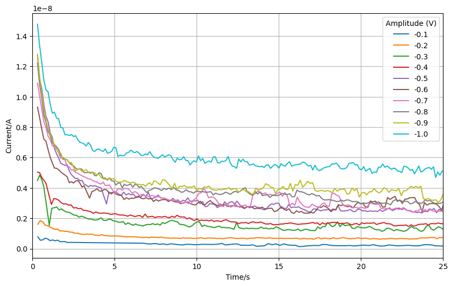
\includegraphics[width=0.6\textwidth]{Chapter5/Figs/b.png}
\caption[The current-time response for a device with a conductive ITO top electrode.]{The current-time response for a device with a conductive ITO top electrode. The current is generated in response to a step potential applied to the top contact with respect to the bottom. It exhibits only the increase in conductance and not the decrease. As the current increases, the noise level also rises until the device reaches a point of breakdown. The structure of the device is identical to that of the gold-contacted devices, with the exception of the change in the top electrode's material from gold-titanium to indium tin oxide (ITO).}
\label{fig:5b}
\end{figure}

\noindent Devices fabricated with a conductive ITO top electrode, in lieu of the gold-titanium contact, do not exhibit the anticipated decay in conductance; rather, they display only the initial increase. Figure \ref{fig:3h} illustrates the current-time response of an ITO-contacted device. As observed previously in the gold devices, the current begins to increase; however, it never reaches the inflection point. Instead, it continues to increase in conductance, becoming progressively noisier until the device undergoes breakdown.\\

\noindent The ITO device has undergone a comparable stressing process to that of the gold devices, which is outlined in the preceding chapter. In the initial stages, the devices exhibit only capacitive currents and possess a very high resistance. Subsequently, a constant current stressing procedure is employed to produce a more conductive device. \\

\noindent Following a period of relaxation, a repeatable transient is produced, provided that the applied voltage is maintained for a sufficiently brief duration to prevent breakdown of the device. A comparable phenomenon has been documented \cite{moon2019rram} in a variety of oxides and is frequently employed in the replication of short-term potentiation of synapses \cite{zhang2017emulating, chang2011short}.\\

\noindent Furthermore, this absence of slower dynamics may corroborate with previous findings \cite{meyer2005oxygen}, where the slower dynamics were postulated to be attributable to oxygen vacancies. It is conceivable that the ITO contact is more prone to exchange oxygen with the oxygen vacancy than the inert gold contact. \\

\begin{figure}[htbp!] 
    \centering    
    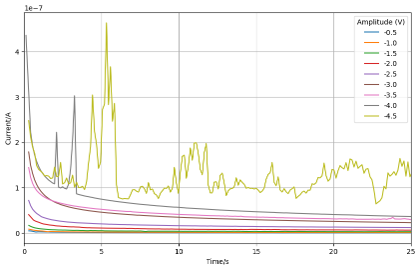
\includegraphics[width=0.6\textwidth]{Chapter5/Figs/c.png}
    \caption[instabilities of potentiation and depression on the amplitude of applied voltage pulses.]{instabilities of potentiation and depression on the amplitude of higher applied voltage pulses on ITO devices.}
    \label{fig:5c}
\end{figure}

\noindent An alternative hypothesis is that the Au contact is diffusing through the oxide, whereas the ITO contact is not. Previous observations have shown that Au can form conductive bridges between two contacts through a thin film of $ZnO$ \cite{peng2012resistive}. Given that gold is known to diffuse in silicon dioxide films, this could be a possibility \cite{madams1974migration}. However, TEM analyses of the devices studied in this thesis have not produced observable gold filaments, casting doubt on this hypothesis \cite{mehonic2017intrinsic}.\\


\noindent An additional potential explanation for the observed discrepancy in behaviour between the Au and ITO contacts is the possibility of differences in their respective work functions. While not directly measured on the samples in question, the work function of gold is reported to be between 4.9 and 5.2 electronvolts (eV) \cite{tran2019anisotropic}, while thin films of indium tin oxide (ITO) have been measured to have a work function between 4.25 and 4.28 eV \cite{schlaf2001work}. \\

\noindent This could result in a difference in work function of approximately 1 eV. Such differences would lead to offsets in the band alignments at the contact and oxide, which could affect which traps within the oxide the electrons are injected into. As discussed in the previous chapter, the disappearance of the slower decay in conductance with the change in top electrode is suggestive of proton migration playing a role in the slower decay in device current.

\section[Empirical Model Fitting]{Empirical Model Fitting}

This section presents the development of empirical models designed to track the rates of increase and decrease in conductance separately. The models are primarily intended to quantify the rate of change in conductance. The question of a physical model will be addressed in the following section.

\subsection[Evaluation Approach]{Evaluation Approach}

\noindent The models explored here are derived from the relaxation experiments that were previously outlined in the preceding chapter. It was evident that the gradual decline in device current delineated the upper limit of the maximum device current, while the initial surge in current approached this maximum but did not exceed it. 
\begin{align}
I(t) = f_{inc}(t) \times f_{dec}(t) \quad \forall \left\{ f_{inc}(t) \in [0 \to 1] : f_{dec}(t) \in \mathbb{R} \right\} \label{eq:5.1}
\end{align}

\noindent This is represented by the product of two time-dependent functions, $f_{inc}(t)$ and $f_{dec}(t)$. The increase in current is analogous to a charging term, $f_{inc}(t)$, which rises from 0 to 1. Initially, this function defines the device current. However, as $f_{inc}(t)$ approaches 1, it then allows the function it is multiplied with to define the total current, in this case  $f_{dec}(t)$. \\

\noindent Although this equation forms the basis of the empirical model, questions remain regarding the specific forms that $f_{inc}(t)$ and $f_{dec}(t)$ should take and the most appropriate means of comparing their effectiveness. The efficacy of each fitting equation is evaluated based on two criteria: the quality of the fit and the degree of realism of the fitted parameters in relation to the underlying physical system from which the model is derived.\\

\noindent The correspondence between each term of a given model and a physical property is contingent upon the physical system from which the model is derived. These properties are assigned a range of values that are deemed realistic. Values outside of this range may indicate that the assumed model is not applicable. The specific correspondence between physical properties and terms is model-specific and will be detailed later in conjunction with the model.\\

\noindent The discrepancy between the fitted equation and the original experimental data is referred to as the residual. This can often be a useful visual indicator of the quality of the fit. An optimal fit would manifest residuals that are centered around zero, exhibiting no systematic offsets or time-variant components. \\

\noindent The residuals in this form indicate that the fitted equation tracks the experimental data well, with the variances in the residuals around zero assumed to be a form of noise or variance in the original data. In contrast, a less optimal fit would exhibit systematic offsets that vary over time. This indicates that either an additional term is absent or the incorrect function has been selected. \\

\noindent However, while residuals are useful for visually assessing a fit, they are less so when larger datasets are being fitted. Therefore, only one residual for each model is assessed, which is representative of the model's performance. The same experimental data will be fitted for each model, thus ensuring an accurate comparison. In order to assess a model's goodness of fit across a whole dataset, a single numerical metric that can quantify the fit is preferred.\\

\noindent A more quantitative description of the goodness of fit is provided by the $R^2$ measure. The $R^2$ measure is a statistical tool that enables the comparison of the variance between the observed data points and the model's predicted values against the variance of the observed data and the mean of that data. In other words, it can be acknowledged that the most straightforward model for predicting a dataset would be to assume the mean value of the dataset in all cases.
\begin{align}
SS_{tot} &= \sum_{i}\left( y_i - \bar y \right)^2 \label{eq:5.2} \\
SS_{res} &= \sum_{i}\left( y_i - f_i \right)^2 \label{eq:5.3} \\
 R^2 &= 1 - \frac{SS_{res}}{SS_{tot}} \label{eq:5.4} 
\end{align}

\noindent In this case, the variance is defined by (\ref{eq:5.2}), Where $y_i$ is an individual datapoint and $\bar y$ is the mean average of the dataset, which is equal to the variance of the dataset. The variance of the dataset against the model's predictions can also be calculated with (\ref{eq:5.3}), Where $f_i$ is model’s predicted value at $i^th$ index, for any other model developed. \\

\noindent If the variance is similar to that of the dataset, the model is no more than a simple mean value predictor, and thus the data fit is poor. An alternative indication of a good fit is provided by a model with a variance much less than that of the dataset. However, residuals should still be checked. The $R^2$ value shown in (\ref{eq:5.4}), defined by the ratio of the variance of the model to the variance of the dataset, is based on this premise and increases as the model's fit improves.\\

\noindent Notwithstanding the possibility of attaining an optimal fit, the values of the fitted parameters remain uncertain. To illustrate, a minimum in the fitting error could be achieved by a range of parameter values. This range is referred to as the confidence bounds, which can be interpreted as the range within which the fitting algorithm is certain the final value lies. \\

\noindent For example, 90\% confidence bounds will define a range within which the algorithm is 90\% sure the optimal value can be found. If a higher confidence is required, the range will generally increase. Consequently, there is a trade-off between certainty and specificity. In this work, the standard confidence threshold of 90\% was employed.\\

\noindent The choice of model for a particular dataset is influenced by the magnitude of the confidence intervals. If a model results in fitted parameters with large confidence intervals, it can present a challenge when interpreting the results, particularly if the changes in these values are small. Consequently, when selecting a model for the analysis of a dataset, preference will be given to models with smaller intervals.


\subsection[Model Definition]{Model Definition}

The current transients observed in amorphous silicon oxide devices appear to result from two distinct changes occurring within the device simultaneously, leading to both an increase and a decrease in conductance. The two changes in conductance exhibit a number of distinguishing characteristics. \\

\noindent Firstly, the increase in conductance occurs significantly faster than the subsequent decay. Secondly, in terms of volatility, the increase in conductance relaxes to its initial state within tens of milliseconds, whereas the decay in conductance can take hours to fully reset. Thirdly, in terms of their material dependence, the decay in conductance can be removed by changing the material of the electrodes \cite{mannion2022current}. \\

\noindent This has led to the conclusion that the two changes are driven by different mechanisms and can exist in isolation, which will be detailed in the following sections. The SPICE models for each of these processes will first be presented separately, and then the two will be combined to obtain the final model.

\begin{figure}[htbp!] 
    \centering    
    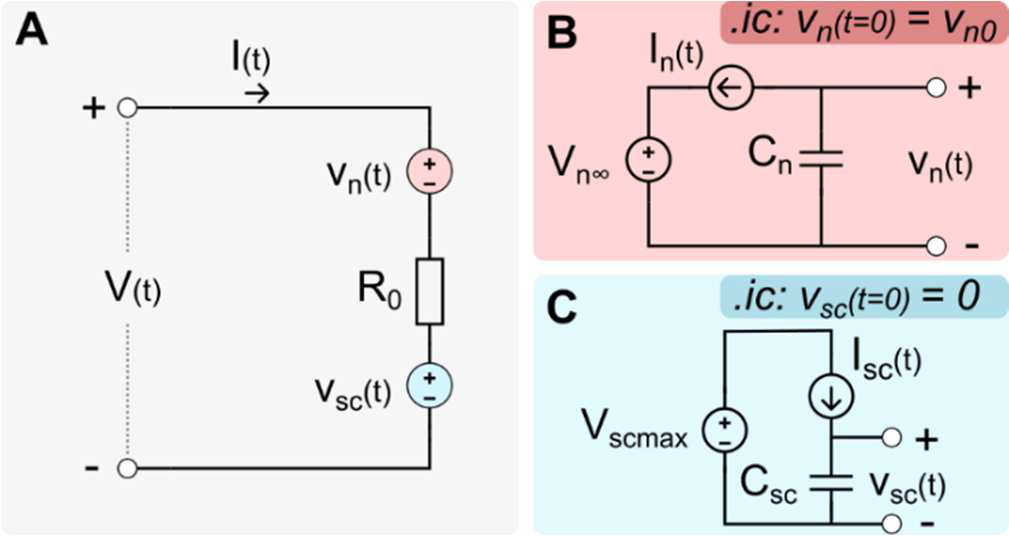
\includegraphics[width=1\textwidth]{Chapter5/Figs/d.png}
    \caption[SPICE Model diagram.]{SPICE Model diagram. The SPICE model generates an output current, \textit{I(t)}, based on an input voltage, \textit{V(t)}. The circuit incorporates a single resistor, $R_0$, along with two diode models that serve to attenuate or amplify the voltage applied to the resistor. These diode models are represented by the sub-circuits highlighted in blue and red.}
    \label{fig:5d}
\end{figure}


\noindent The accelerated rise in conduction appears to be attributable to the phenomenon of charge trapping. This is corroborated by its shorter timescales, greater volatility, and experiments in which optically injected carriers were demonstrated to accelerate the process. One potential mechanism by which charge trapping affects device conductance is through modulation of the height of a Schottky-like barrier \cite{cowley1965surface}, which may be influenced by the population of interface states \cite{sze2021physics}. \\

\noindent Although Schottky barriers are typically formed between metal-semiconductor interfaces, studies have identified analogous barriers within memristor devices \cite{hansen2015double}. The silicon oxide devices exhibit rectifying behaviour, indicating the presence of an interface barrier at one of the metal-insulator interfaces. Additionally, the filaments in the devices are composed of silicon-rich regions within the oxide, suggesting that the interface between these filaments and metal contacts may resemble a Schottky interface.\\

\noindent The Schottky barrier is modelled as a voltage drop, which acts to reduce the voltage across the active layer of the device, as illustrated in \ref{fig:5d}. As the height of the Schottky barrier diminishes, the potential across the active layer increases, resulting in a greater device current. The voltage drop resulting from the Schottky-like barrier is a function of time and is modelled using the sub-circuit illustrated in red in \ref{fig:5d}. \\

\noindent The magnitude of the voltage drop is represented within the sub-circuit by the voltage across the capacitor, $C_n$. The initial value of the aforementioned variable is discharged by the current source, $V_{n0}$. The rate of discharge is defined by the current source, $I_n(t)$, whose magnitude is proportional to the difference between the current voltage drop across the Schottky barrier and its final equilibrium value, $V_{n\infty}$.
\begin{align}
I_n(t) = \alpha \times \left[ V_n(t) - V_{n\infty} \right] \label{eq:5.5} 
\end{align}

\noindent In this equation, $\alpha$ corresponds to the probability of trapping a carrier, while the voltage difference relates to the concentration of unpopulated states. The current source discharges the capacitor to a final equilibrium voltage, $V_{n\infty}$, where the trapping and de-trapping currents are equal. An additional leaking resistor, $R_{leak}$, is introduced to correctly adjust for the rectifying behaviour of the device.\\

\noindent There is compelling evidence that the observed decline in conductance can be attributed to the movement of charged ions within the oxide thin film. This hypothesis has been put forth in the majority of publications on such current transients \cite{wang2006oxygen}. This is largely based on the observation that the decay in conductance occurs over a time scale of tens to hundreds of seconds, which is too long to be associated with the trapping of electrons or holes. \\

\noindent Furthermore, in accordance with the drifting defect hypothesis, it has been demonstrated that the process can be reversed by applying a voltage of opposite polarity, despite the device exhibiting significantly reduced currents in the opposite polarity. The model adhere to this approach and hypothesise the presence of migrating defects. Of particular significance is the assumption that the ionic current induced by the migrating space charge is negligible in comparison to the electronic currents, as predicted \cite{meyer2005oxygen}. \\

\noindent It is assumed that the electronic current flows through a conductive channel within the oxide. In our silicon oxide devices, this is a silicon-rich filament that forms during electrical stressing. Such filaments are common in memristors and have been observed in our devices using etching C-AFM techniques \cite{buckwell2015conductance}.\\

\noindent In order for an electronic current to be induced through these filaments, it is necessary that a potential be present across the channel. In our model, the migrating space charge modulates the current by reducing the potential experienced along the filament. It is probable that this space charge is a positively charged ion that has accumulated in proximity to the upper gold electrical contact. This assertion is corroborated by the observation that the impact of the accumulation of space charge can be negated by modifying the material of the top electrical contact from gold to indium tin oxide \cite{mannion2022current}.\\

\noindent The precise nature of this ion remains uncertain. A substantial amount of oxygen migration and associated oxygen vacancies have been observed throughout the device when under bias \cite{vanka2022hydrogen}, indicating that this could be a viable candidate. However, in other devices, hydrogen has been identified as a defining factor in device behaviour. Additionally, hydrogen has been detected in significant quantities within our devices \cite{lagarias1998convergence}. Given the lack of certainty regarding the identity of the ion, we assume a generic space charge.\\

\noindent The effect of the space charge on the conductive channel can be described as follows. In the initial phase, the space charge exhibits a homogeneous distribution. Upon the application of a voltage to the device, a force is imparted on the space charge, resulting in its drift and accumulation at the device electrode. This accumulation effectively blocks the space charge from exiting the oxide.  \\

\noindent This accumulation results in the formation of a region of higher space charge concentration, which consumes a portion of the potential applied across the device. This results in a reduction in the potential drop across the conductive channel. As the space charge accumulates, this voltage drop increases, meaning less potential is dropped across the channel and a reduction in device current is observed. \\

\noindent Eventually, the drifting force imparted on the space charge will reach equilibrium with the diffusion and Coulombic repulsion formed by the accumulated space charge, leading to a steady state condition. When the potential is removed, the space charge diffuses back to its original distribution. \\

\noindent The aforementioned process is modelled using the circuit illustrated in Figure \ref{fig:5d}. The conductive channel is represented by a fixed resistance, designated as $R_0$. The voltage across the conductive channel is defined by the applied potential at the terminals of the device, $V(t)$, and the voltage source, $V_{sc}(t)$, which represents the voltage drop caused by the accumulated space charge. This voltage source is time-dependent and is defined by the subcircuit shown in blue. As the voltage of this source increases over time, the voltage across the fixed resistor drops and the device current also reduces.
\begin{align}
I_{sc}(t) = \left[ V_{scmax} - V_{sc}(t) \right] \times \left[ \mu \left( V(t) - V_{sc}(t) \right) \right] \label{eq:5.6} 
\end{align}

\noindent The blue sub-circuit illustrated in \ref{fig:5d} is responsible for monitoring the accumulation of the space charge and its corresponding voltage drop, which is represented by the voltage across the capacitor $C_{sc}$. The capacitor is charged by the current source, $I_{sc}(t)$, which generates a current in (\ref{eq:5.6}). The capacitor is defined by the voltage applied across the device and $\mu$, which symbolises the mobility of the space charge. The current source draws charge from a voltage source representing the steady-state voltage drop, i.e. the maximum voltage drop consumed by the accumulated space charge $V_{scmax}$.
\begin{align}
I_d(t) = \left( I_0 + I_{\delta} V_n(t) \right)\times \left( e^{\frac{V(d_1,d_2)}{nV_t} }  - 1\right) \label{eq:5.7}
\end{align}

\noindent To complete the model, the subcircuits for both potential drops are combined as illustrated (\ref{eq:5.7}). The two voltage drops act upon a single resistor representing the conductive channel, $R_0$. In practice, this channel does not exhibit ohmic conduction and thus its resistance will have a voltage dependence. This is taken into account while collecting the meta-parameters.

\section[The Combined Model]{The Combined Model}

\subsection[Parameter Fitting]{Parameter Fitting}

\subsection[Model Performance]{Model Performance}

\section[Summary]{Summary}

\noindent Neuromorphic modelling is concerned with the creation of artificial systems that emulate the functionality of biological neural systems, particularly in terms of their physical implementation. The term was first used in the late 1980s to describe digital and analogue hardware that is organised in a more brain-like manner than traditional computer hardware \cite{mead1990neuromorphic}. \\

\noindent One of the fundamental concepts underlying neuromorphic systems is parallel distributed processing. Neuromorphic systems arrange computations at the neural level, with a specific focus on facilitating rapid communication between neural processing units. This contrasts with other parallel distributed systems, such as graphics processing units (GPUs), which are typically optimized for independent parallel computations and exhibit limited communication between units. \\